\begin{savequote}[120mm]
Each gesture is created at the moment of speaking and highlights what is
relevant and the same entity can be referred to by gestures that have changed
their form.
\qauthor{David McNeill, \textit{Hand and mind: what gestures reveal about
thought}}
\end{savequote}
\chapter{Gesture Interaction}
This chapter discusses application level consideration for natural multimodal
interaction.

\section{Server Client Architecture}
I developed a multimodal input recognition engine that consists of a gesture
recognition engine and a speech recognition engine. The gesture recognition
engine includes the hand tracking, feature extraction and gesture recognition
modules described in the previous chapters.
For speech recognition, I used the application programming interface (API) from
the Windows for Kinect SDK\footnote{\url{http://msdn.microsoft.com/en-us/library/jj131035.aspx}}.

The multimodal input recognition engine runs as a server sending recognized
gesture and speech events over a WebSocket\footnote{http://en.wikipedia.org/wiki/WebSocket}. Any client
application can subscribe to the input events by connecting to the server
socket. There are two types of events: gesture and speech, and they are
serialized in JSON format\footnote{\url{http://www.json.org/}}
(Listing~\ref{lst:gesture} and~\ref{lst:speech}).

\begin{lstlisting}[caption={Gesture event JSON object}, label={lst:gesture}]
{"gesture": <gestureName>, 
 "type": <"StartPreStroke" | "StartGesture" | "StartPostStroke">,
 "stage": <"PreStroke" | "Gesture" | "PostStroke">,
 "rightX": <rightHandXWorldCoordinate>,
 "rightY": <rightHandYWorldCoordinate> } 
\end{lstlisting}

\begin{lstlisting}[caption={Speech event JSON object}, label={lst:speech}]
{"speech": <speechTag>}
\end{lstlisting}

\section{Gesture Controlled Presentation}
To demonstrate the use of multimodal input recognition system in a real life
application, I developed a gesture controlled presentation
application\footnote{See
\url{http://groups.csail.mit.edu/mug/projects/gesture_kinect/} for demo
videos.}, acting as a client. The presentation application is HTML based using
the \texttt{reveal.js} framework\footnote{\url{http://lab.hakim.se/reveal-js/}}.
The framework's API allows me to directly perform functionalities related to
presentation such as changing slides, showing overview, and pausing slide
show instead of controlling the presentation by binding to mouse events which is
commonly done in many previous hacks demonstrating gesture control. I believe
that by mimicking mouse events, one limits the full potential of
gesture input.

\subsection{Handling Different Types of Gestures}
In this application, I demonstrate the use of path and pose gestures, and how
the system respond differently for discrete flow and continuous flow gestures. I
map the gestures in the YANG dataset to presentation control actions
(Table~\ref{tab:map-gesture}). 

\begin{table}[tbh]
\centering
\begin{tabular}{|l|l|}
\hline
\thead{Gesture} & \thead{Action} \\
\hline
Swipe Left & Next slide (DF) \\
\hline
Swipe Right & Previous slide (DF) \\
\hline
Circle & Toggle overview (show all slides) (DF) \\
\hline
Horizontal Wave & Toggle pause (turn screen black) (DF) \\
\hline
Point & Show a round cursor corresponding to hand position (CF) \\
\hline
Palm Up & Show a square cursor and seek video forward or backward (CF) \\
\hline
\end{tabular}
\caption{Mapping from gestures to presentation control actions. DF stands for
discrete flow gesture and CF stands for continuous flow gesture.}
\label{tab:map-gesture}
\end{table}

An interface
should reflect the system's current state of understanding of users'
actions to help users develop the right mental model for interaction. For
discrete flow gestures, the interface needs to respond at the StartPostStroke
event. This responsiveness of the system helps users understand the relation
between their actions and the system's responses. For continuous gestures, the
interface needs to show visual feedback of frame by frame changes
corresponding to certain hand input parameters. In addition, as pose gestures
have distinct poses but arbitrary movement, it is important to have different 
visualization to show the system's understanding of the different
poses. Hence, for Point gesture, the system shows a round cursor moving
according to the user's hand position, and for Palm Up gesture, it shows a
square cursor (Figure~\ref{fig:palm-up}).
Listing~\ref{lst:gesture} shows the corresponding client code in CoffeeScript.

\begin{figure}[tbh]
\centering
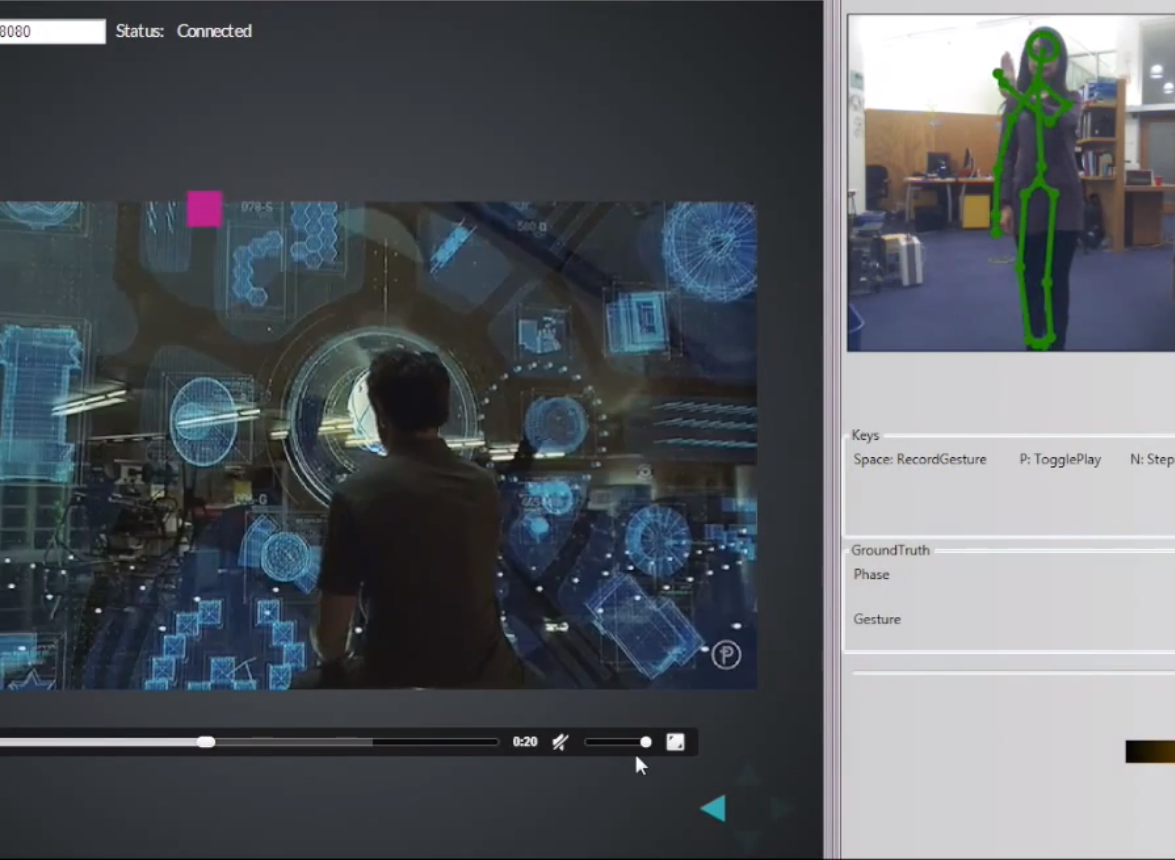
\includegraphics[trim=0 2.7cm 0 0,
clip, width=\columnwidth]{figures/video_control.PNG}
\caption{Square cursor for Palm Up gesture to seek video forward or backward by
moving hand left or right.}
\label{fig:palm-up}
\end{figure}

\begin{lstlisting}[caption={Client code mapping gesture events to actions.},
label={lst:client-code}] 
switch ge.eventType
  when 'StartPostStroke'
    switch ge.gesture
      when 'Swipe_Left' then Reveal.right()
      when 'Swipe_Right' then Reveal.left()
      when 'Circle' then Reveal.toggleOverview()
      when 'Horizontal_Wave' then Reveal.togglePause()
  else
    switch ge.gesture
      when 'Point' then @_view.updateCirclePointer(ge.rightX, ge.rightY)
      when 'Palm_Up' then @_view.updateSquarePointer(ge.rightX, ge.rightY)
      when 'Rest' then @_view.reset()
\end{lstlisting}

\subsection{Gesture and Speech}
Traditionally, gestures are used to augment speech in interaction, as pioneered
by Bolt's ``Put That There'' system \cite{Bolt80}. My previous user study
\cite{yin10thesis} show that speech also can augment gestures.

When using gesture to augment speech, gesture is often used to indicate
location. This type of gesture is called deictic gesture (pointing gesture)
which is very effective to convey spatial information, and is often used to
supplement a spoken deictic marker (this, those, here, etc.)~\cite{oviatt97}. In
my application, the user can show a slide by pointing at it in the overview and
say ``show this slide'' (Figure~\ref{fig:point-overview}). Synonyms can be used
as well to improve flexibility and naturalness.

\begin{figure}[tbh]
\centering
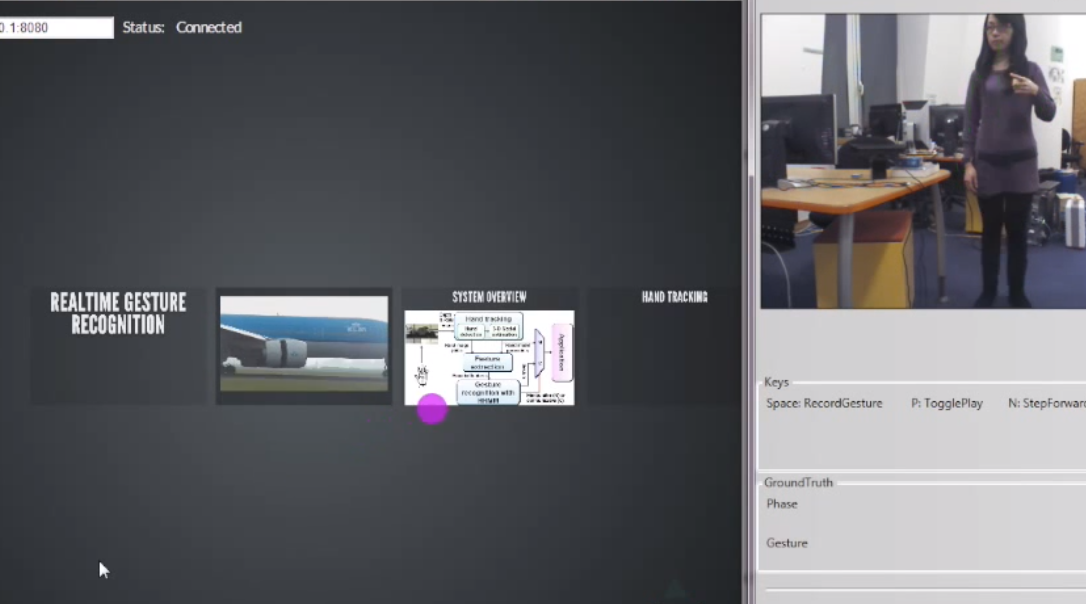
\includegraphics[width=\columnwidth]{figures/point_overview.PNG}
\caption{In the overview mode, user can point to a slide and say ``show this
slide'' to display it.}
\label{fig:point-overview}
\end{figure}

When speech is used to augment gesture, the spoken words are adjectives and
adverbs to modify actions indicated by gestures~\cite{yin10thesis}. This
combination is particularly useful when there is a limitation in the
expressiveness of the gesture or in the physical space of the gesture. In my
application, the user can say ``faster'' or ``slower'' or their synonyms to
control speed when they use the Palm Up gesture to seek video forward and
backward.

The speech recognition is based on key word spotting by defining grammars in
XML (Listing~\ref{lst:grammar}). All synonyms are recognized as the same speech
tag, and the application needs to define behavior according to the speech tags. In my application, the behavior to speech
events is dependent on gesture event as well (see
Listing~\ref{lst:speech-code}).

\begin{lstlisting}[caption={An example of grammar definition in XML.},
language=XML, label={lst:grammar}] 
<item>
  <tag>SHOW</tag>
  <one-of>
    <item>show</item>
    <item>open</item>
    <item>display</item>
    <item>go to</item>
  </one-of>
</item>
\end{lstlisting}

\section{Discussion}
The server client architecture provides a clean separation of the user
interface and the backend recognition engine, hiding the complexity of the
multimodal input recognition from application developers. The gesture event
based API gives a rich set of input compared to the mouse events, and allows
easy mapping to application functionality.

\begin{lstlisting}[caption={Code for speech events.}, label={lst:speech-code}]
switch speechText
  when 'MORE'
    @_view.onMore() if @_currentGesture is 'Palm_Up'
  when 'LESS'
    @_view.onLess() if @_currentGesture is 'Palm_Up'
  when 'SHOW'
    @_view.onShowSlide() if @_currentGesture is 'Point'
\end{lstlisting}

%user adaptation
